\documentclass[a4paper, 11pt]{article}

\usepackage[a4paper,margin=1in]{geometry}
\usepackage[english]{babel}
\usepackage[utf8]{inputenc}
\usepackage[T1]{fontenc}
\usepackage{lmodern}
\usepackage{listings}
\usepackage{graphicx}
\usepackage{amsmath}
\usepackage{framed}
\usepackage{amsfonts}
\usepackage{caption}
\usepackage{subcaption}
\usepackage{listings}
\usepackage{tabularx}
\usepackage{color}
\usepackage[dvipsnames]{xcolor}
\usepackage{fancyhdr}
\usepackage{lastpage}
% \usepackage[round, sort]{natbib}
\usepackage{tikz}

\bibliographystyle {abbrv}
\usetikzlibrary{decorations.pathreplacing, matrix}


\graphicspath{{../imgs/}}
\interlinepenalty=10000

\definecolor{morange}{RGB}{237,106,90}
\definecolor{mgreen}{RGB}{63,127,95}
\definecolor{mpurple}{RGB}{127,0,85}

\lstset{
  basicstyle=\small\ttfamily, % Global Code Style
  captionpos=b, % Position of the Caption (t for top, b for bottom)
  extendedchars=true, % Allows 256 instead of 128 ASCII characters
  tabsize=2, % number of spaces indented when discovering a tab
  columns=fixed, % make all characters equal width
  keepspaces=true, % does not ignore spaces to fit width, convert tabs to spaces
  showstringspaces=false, % lets spaces in strings appear as real spaces
  breaklines=true, % wrap lines if they don't fit
  frame=trbl, % draw a frame at the top, right, left and bottom of the listing
  frameround=tttt, % make the frame round at all four corners
  framesep=4pt, % quarter circle size of the round corners
  numbers=left, % show line numbers at the left
  numberstyle=\tiny\ttfamily, % style of the line numbers
  commentstyle=\color{mgreen}, % style of comments
  keywordstyle=\color{mpurple}, % style of keywords
  stringstyle=\color{morange}, % style of strings
}

% TAILLE DES PAGES (A4 serré)

\setlength{\intextsep}{2em}
\setlength{\parindent}{0pt}
\setlength{\parskip}{1em}
%% \setlength{\textwidth}{17cm}
%% \setlength{\textheight}{24cm}
%% \setlength{\oddsidemargin}{-.7cm}
%% \setlength{\evensidemargin}{-.7cm}
%% \setlength{\topmargin}{-.5in}


\pagestyle{fancy}
\renewcommand{\headrulewidth}{0pt}
\renewcommand{\footrulewidth}{0.6pt}% default is 0pt
\lhead{}
\rhead{}
\lfoot{Page \thepage\ of \pageref{LastPage}}
\rfoot{Rémi Lespinet}
\cfoot{}
\cfoot{}

\newcounter{cquestion}
\renewcommand{\thecquestion}{\arabic{cquestion}}
\newenvironment{question}
{\par \vspace{0.5em} \noindent \stepcounter{cquestion} \hspace{-1em}
 $\bullet$ \underline{Q\thecquestion :}}
{}

\newenvironment{note}
{\begin{framed} \textbf{Note : }}
{\end{framed}}


% Commandes de mise en page
\newcommand{\file}[1]{\lstinline{#1}}
\newcommand{\name}[1]{\emph{#1}}
\newcommand{\Fig}[1]{Fig \ref{#1} p. \pageref{#1}}
\newcommand{\Figure}[1]{Figure \ref{#1} p. \pageref{#1}}
\newcommand{\Tab}[1]{Tab \ref{#1} p. \pageref{#1}}
\newcommand{\Table}[1]{Table \ref{#1} p. \pageref{#1}}
\newcommand{\itemi}{\item[$\bullet$]}
% Commandes color
\newcommand{\colgood}[1]{\color{ForestGreen} #1}
\newcommand{\colbad}[1]{\color{BrickRed} #1}


% Commandes de maths
\newcommand{\function}[3]{#1 : #2 \to #3}
\newcommand{\intn}[2]{\left\{ #1 \dots #2 \right\}}
\newcommand{\intr}[2]{\left[ #1 ; #2 \right]}
\newcommand{\intro}[2]{\left] #1 ; #2 \right[}
\newcommand{\dotp}[2]{\langle #1, #2 \rangle}
\newcommand{\logn}[1]{\ln\left( #1\right)}
%% \newcommand{\det}[1]{\left| #1 \right|}
\newcommand{\pd}[2]{\frac{\partial #1}{\partial #2}}
\newcommand{\norm}[1]{\|#1\|}
\newcommand{\set}[2]{\left\{ #1 \hspace{.5em} ; \hspace{.5em}#2 \right\}}
\newcommand{\tr}[1]{Tr\left( #1 \right)}
\newcommand{\pcond}[2]{p(#1 \hspace{-.2em}\mid\hspace{-.2em} #2)}
\newcommand{\picond}[2]{\pi(#1 \hspace{-.2em}\mid\hspace{-.2em} #2)}
\newcommand{\parampicond}[3]{\pi_{#1}(#2 \hspace{-.2em}\mid\hspace{-.2em} #3)}
\newcommand{\e}[1]{\mathop{\mathbb{E}}\left[#1\right]}
\newcommand{\gradwrt}[2]{\nabla_{#1}{#2}}


\newcommand{\iid}{i.i.d }
\newcommand{\wrt}{w.r.t }

% Commandes informatique
\newcommand{\pfun}[1]{{\textbf{\texttt{#1}}}}

\newcommand{\ipart}[1]{\vspace{0.5em}\textbf{#1}\vspace{0.5em}}



\pagenumbering{arabic}

\title{\textsc{Reinforcement learning - MVA 2017/2018 \\ \emph{Homework 2}} }
\author{Rémi Lespinet}
\date{}

\begin{document}

\maketitle
\thispagestyle{fancy}

\section{On-Policy Reinforcement Learning with Parametric Policy}

\begin{question}
  If we condider the gaussian policy
  \begin{displaymath}
    \picond{a}{s} = \dfrac{1}{\sigma_w(s) \sqrt{2 \pi}} e^{-\frac{(a - \mu_{\theta})^2}{2 \sigma_w^2(s)}}
  \end{displaymath}
  we can also write the derivative of the logarithm w.r.t $w$ as
  \begin{displaymath}
    \gradwrt{w}{\log{\picond{a}{s}}} = \dfrac{(a - \mu_{\theta}(s))^2 - \sigma_{w}^2 }{2 \sigma_w^4(s)} \gradwrt{w}{\sigma_{w}^2}(s)
  \end{displaymath}
  This is the version that I use in my code (I define $\sigma^2(s)$
  and $\gradwrt{w}{\sigma_{w}^2}(s)$ directly).

  \subsection{Constant step}

  In this part, we use a constant step $\alpha$. As we can see,
  high values of $\alpha$ make the computation of the estimated
  expected discount reward
  \begin{displaymath}
     \hat{\nabla_{\theta}}(J) = \dfrac{1}{N} \sum_{n = 1}^N \sum_{t = 0}^T \gradwrt{\theta}{\log{\parampicond{\theta}{a_t^{n}}{s_t^{n}}}} R(\tau^n)
  \end{displaymath}
  diverge. Hence $\alpha$ must be chosen very carefully.  The figure
  \ref{fig:constant-step} presents the evolution of the mean parameter
  $\theta$ and the estimated policy performance as a function of the
  number of iteration for the REINFORCE algorithm with constant step
  for different values of the learning rate. In practice the highest
  values of the learning rate do not converge every time and I've
  restarted the simulation in order for them to work. These curves are
  averaged over 5 runs of the algorithm for $N = 100$ samples per
  estimation of the gradient of the policy performance, $T = 100$
  (length of the trajectory) and the $\gamma = 0.9$.

  \begin{figure}[ht]
    \centering
    \begin{subfigure}[t]{0.48\textwidth}
      \centering
      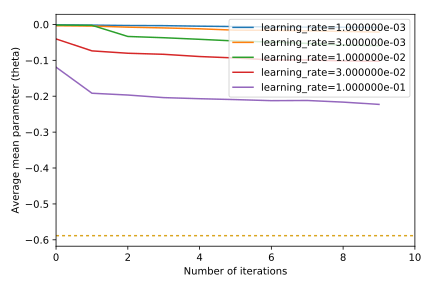
\includegraphics[width=\textwidth]{constant_mean.pdf}
      \caption{Average mean parameter $\theta$}\label{fig:constant-mean.pdf}
    \end{subfigure}
    \quad
    \begin{subfigure}[t]{0.48\textwidth}
      \centering
      \includegraphics[width=\textwidth]{constant_return.pdf}
      \caption{Average return}\label{fig:constant-return.pdf}
    \end{subfigure}
    \caption{Evolution of the mean parameter $\theta$ and the
      estimated policy performance as a function of the number of
      iteration for the REINFORCE algorithm with constant step for
      different values of the learning rate. These curves are averaged
      over 5 runs of the algorithm for $N = 100$, $T = 100$,
      $\gamma = 0.9$. The golden dashed line represents the optimal
      mean parameter value
      $\theta^* = -0.5884$}\label{fig:constant-step}
  \end{figure}

  % \begin{figure}[h!]
  %   \centering
  %     \includegraphics[width=0.7\textwidth]{average_mean_constant.pdf}
  %     \caption{Representation of the arms means and expected
  %       cumulative regret for the second chosen Bernoulli
  %       bandit}\label{fig:average-mean-constant.pdf}
  % \end{figure}

  In our case, a value of $\alpha = 10^{-5}$ seems to work well.  This
  is not surprising to have such order for $\alpha$, in our example,
  we are only interested in the gradient along theta, ($\sigma_w(s)$)
  is constant). If we look at an order of a single MC sample in our
  estimation of the expected discount reward, we see that is is
  expressed as
  \begin{displaymath}
    R(\tau) \sum_{t = 0}^T\nabla_{\theta}{\log{\parampicond{\theta}{a_t}{s_t}}}
    = \dfrac{a_t - \theta s_t}{\sigma_w(s)^2} R(\tau) s_t
  \end{displaymath}
  We know that $a_t$ and $s_t$ are on the order of $10^2$,
  $\sigma_w(s)^ 2 = 0.25$, and $r_t = -\frac{s_t^2 + a_t^2}{2}$ which
  is of the order of $10^4$. Hence a single MC sample in the
  estimation of the expected discount reward should be of the order of
  $10^6$. Since we expect values of $\theta$ to be on the order of
  $1$, we expect the gradient ascend update to be of the order of 1
  \begin{displaymath}
    \theta_{t+1} = \theta_t + \alpha \hat{\nabla_{\theta}}(J)
  \end{displaymath}
  and we must then choose $\alpha$ of the order of $10^{-6}$. In
  practice since the rewards are all negative, the goal of the
  algorithm is to maximize the rewards, which minimizes their absolute
  values and the order of the reward of a trajectory is around
  $10^{3}$ (which explains why we can take sligly larger values for
  $\alpha$).

  \subsection{Adam step}

  The figure \ref{fig:adam-step} presents evolution of the mean
  parameter $\theta$ and the estimated policy performance as a
  function of the number of iteration for the REINFORCE algorithm with
  Adam step for different values of the learning rate (with
  $\beta_1 = 0.9$, $\beta_2 = 0.999$, $\epsilon = 10^{-8}$ as
  recommended). We see that this stepping strategy works really well
  in practice when compared to the other tested methods.

  \begin{figure}[ht]
    \centering
    \begin{subfigure}[t]{0.48\textwidth}
      \centering
      \includegraphics[width=\textwidth]{adam_mean.pdf}
      \caption{Average mean parameter $\theta$}\label{fig:adam-mean.pdf}
    \end{subfigure}
    \quad
    \begin{subfigure}[t]{0.48\textwidth}
      \centering
      \includegraphics[width=\textwidth]{adam_return.pdf}
      \caption{Average return}\label{fig:adam-return.pdf}
    \end{subfigure}
    \caption{Evolution of the mean parameter $\theta$ and the
      estimated policy performance as a function of the number of
      iteration for the REINFORCE algorithm using the \textbf{Adam}
      stepping algorithm for different values of the learning
      rate. These curves are averaged over 5 runs of the algorithm for
      $N = 100$, $T = 100$, $\gamma = 0.9$. The golden dashed line
      represents the optimal mean parameter value
      $\theta^* = -0.5884$}\label{fig:adam-step}
  \end{figure}

  % In this implementation, a state is an array constitued of a single
  % element. Even if in this homework a state is always a scalar, I
  % assume that a state can be a vector, and hence I cast it into a
  % scalar when it is absolutely needed to do so (e.g in the Mean and
  % variance computation functions)

  \newpage
  \subsection{Other strategies}

  I've also implemented a discounted strategy, where
  \begin{displaymath}
    \alpha_t = \gamma^t \alpha_0
  \end{displaymath}
  The figure \ref{fig:mixed-step} presents the different methods that
  we have seen.

  \begin{figure}[h!]
    \centering
    \begin{subfigure}[t]{0.48\textwidth}
      \centering
      \includegraphics[width=\textwidth]{mixed_mean.pdf}
      \caption{Average mean parameter $\theta$}\label{fig:mixed-mean.pdf}
    \end{subfigure}
    \quad
    \begin{subfigure}[t]{0.48\textwidth}
      \centering
      \includegraphics[width=\textwidth]{mixed_return.pdf}
      \caption{Average return}\label{fig:mixed-return.pdf}
    \end{subfigure}
    \caption{Evolution of the mean parameter $\theta$ and the
      estimated policy performance as a function of the number of
      iteration for the REINFORCE algorithm for different stepping
      strategies. These curves are averaged over 5 runs of the
      algorithm for $N = 100$, $T = 100$,
      $\gamma = 0.9$}\label{fig:mixed-step}
  \end{figure}

  A lot of stepping strategy rely on the ability to compute the
  function to be optimized in several points (for example backtracking
  line search). In this case, we cannot compute the function easily,
  and it needs to be estimated by Monte Carlo sampling which make
  these stepping strategies relatively costly.



\end{question}

\begin{question}
  We are interested in the behavior of the REINFORCE algorithm when
  the number of MC samples $N$ vary. Figure \ref{fig:N-comparison} represents the
  evolution of the mean parameter $\theta$ and the estimated policy
  performance for different values of $N$ as a function of the
  % The figure \ref{} represents the evolution of the mean parameter
  % $\theta$ and the estimated policy performance when we vary the
  % number of MC samples $N$. These are plotted as a function of
  total number of trajectories computed $N K$ (where $K$ is the number
  of iteration of the algorithm e.g the number of time that the
  parameter $\theta$ is updated). We use the Adam stepping strategy
  with a learning rate of $0.1$ to make this comparison.


  \begin{figure}[ht]
    \centering
    \begin{subfigure}[t]{0.48\textwidth}
      \centering
      \includegraphics[width=\textwidth]{N_mean.pdf}
      \caption{Average mean parameter $\theta$}\label{fig:N-mean.pdf}
    \end{subfigure}
    \quad
    \begin{subfigure}[t]{0.48\textwidth}
      \centering
      \includegraphics[width=\textwidth]{N_return.pdf}
      \caption{Average return}\label{fig:N-return.pdf}
    \end{subfigure}
    \caption{Evolution of the mean parameter $\theta$ and the
      estimated policy performance as a function of the total number
      of iterations $N K$ for the REINFORCE algorithm for different
      values of $N$. These curves are averaged over 5 runs of the
      algorithm an use Adam stepping strategy with $\alpha = 0.01$.
      $T = 100$, $\gamma = 0.9$}\label{fig:N-comparison}
  \end{figure}

  As we can see, when we estimate the gradient of the policy
  performance with a low number of sample, we obtain a very noisy
  approximation, but it allows to do a lot more policy parameter
  updates for a given amount of computation time.

\end{question}

\section{Off-Policy Reinforcement Learning with Value Function Approximation}

\begin{question}
  The estimate state value function is parametrized by
  \begin{displaymath}
    \hat{Q}_\theta (s, a) = a \theta_1 + s a \theta_2 + (s^2 + a^2) \theta_3
  \end{displaymath}
  (see \verb+LinearSecondOrderQModel+ in the notebook)

  As suggested, I've chosen a behavioral policy that choses actions
  uniformly in the action space (see \verb+UniformPolicy+) to collect
  the dataset. I simulate $50$ trajectories of length $50$ using this
  policy. The figure \ref{fig:Q-comparison} compares the state
  value function obtained (state and action have been discretized over
  a $20 \times 20$ grid), and the optimal state value function
  (provided). The figure \ref{fig:fqi-performance} shows the evolution
  of the estimated policy performance learnt with the FQI algorithm as
  a function of the number of the iterations.

  \begin{figure}[h!]
    \centering
    \begin{subfigure}[t]{0.48\textwidth}
      \centering
      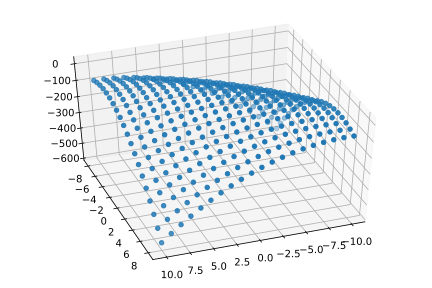
\includegraphics[width=\textwidth]{Q_fqi.pdf}
      \caption{Representation of the Q function obtained by
        FQI}\label{fig:Q-fqi.pdf}
    \end{subfigure}
    \quad
    \begin{subfigure}[t]{0.48\textwidth}
      \centering
      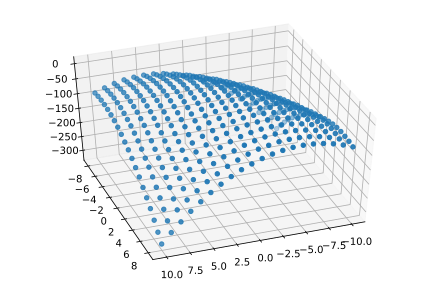
\includegraphics[width=\textwidth]{Q_optimal.pdf}
      \caption{Representation of the optimal Q function
        (provided)}\label{fig:Q-optimal.pdf}
    \end{subfigure}
    \caption{Comparison of the state value function obtained with the
      optimal one (states and actions are discretized over a
      $20 \times 20$ grid}\label{fig:Q-comparison}
  \end{figure}


  Note that at each iteration, we use the whole dataset collected, as
  the size of the dataset increases, it could be intractable, and we
  should use random subsets of the dataset.

  % The table \ref{tab:comp-performance} reports the policy
  % performance obtained with REINFORCE algorithm and FQI algorithm.

  % \begin{table}[h!]
  %   \centering
  %   \begin{tabular}{|c|c|c|}
  %     \hline
  %     \textbf{REINFORCE} & \textbf{FQI} & \textbf{Optimal} \\
  %     \hline
  %     & & \\
  %     \hline
  %   \end{tabular}
  %   \captionof{table}{Representation of the transition table
  %     corresponding to the graph} \label{tab:transition-table}
  % \end{table}

  As we can see the FQI algorithm converges really fast and gives a
  good approximation of the state value function (in this case the
  optimal state value function is well described by a second order
  polynomial in $(s, a)$).

  \begin{figure}[h!]
    \centering
    \includegraphics[width=0.6\textwidth]{fqi_performance.pdf}
    \caption{Representation of the performance of the policy as the
      number of iteration in the FQI algorithm
      increases.}\label{fig:fqi-performance}
  \end{figure}

\end{question}


\end{document}

%% \begin{figure}[p]
%%   \centering
%%   \begin{subfigure}[t]{0.40\textwidth}
%%     \centering
%%     \includegraphics[width=\textwidth]{LDA_classificationA_train}
%%     \caption{Training observations A ($150$ points)}\label{fig:LDA-A-train}
%%   \end{subfigure}
%%   \quad
%%   \begin{subfigure}[t]{0.40\textwidth}
%%     \centering
%%     \includegraphics[width=\textwidth]{LDA_classificationA_test}
%%     \caption{Test observations A ($1500$ points)}\label{fig:LDA-A-test}
%%   \end{subfigure}
%%   \vskip\baselineskip
%%   \begin{subfigure}[t]{0.40\textwidth}
%%     \centering
%%     \includegraphics[width=\textwidth]{LDA_classificationB_train}
%%     \caption{Training observations B ($150$ points)}\label{fig:LDA-B-train}
%%   \end{subfigure}
%%   \quad
%%   \begin{subfigure}[t]{0.40\textwidth}
%%     \centering
%%     \includegraphics[width=\textwidth]{LDA_classificationB_test}
%%     \caption{Test observations B ($1500$ points)}\label{fig:LDA-B-test}
%%   \end{subfigure}
%%   \vskip\baselineskip
%%   \begin{subfigure}[t]{0.40\textwidth}
%%     \centering
%%     \includegraphics[width=\textwidth]{LDA_classificationC_train}
%%     \caption{Training observations C ($150$ points)}\label{fig:LDA-C-train}
%%   \end{subfigure}
%%   \quad
%%   \begin{subfigure}[t]{0.40\textwidth}
%%     \centering
%%     \includegraphics[width=\textwidth]{LDA_classificationC_test}
%%     \caption{Test observations C ($1500$ points)}\label{fig:LDA-C-test}
%%   \end{subfigure}
%%   \caption{Sample data and decision boundary representation for the LDA classifier on the three files}\label{fig:LDA}
%% \end{figure}




  % \begin{table}[h!]
  %   \centering
  %   \begin{tabular}{|c|c|c|c||c|c|c|}
  %     \hline
  %     & \multicolumn{3}{c||}{\textbf{a0}} & \multicolumn{3}{c|}{\textbf{a1}}\\
  %     \hline
  %     & s0 & s1 & s2 & s0 & s1 & s2 \\
  %     \hline
  %     s0 & 0.45 & 0.00 & 0.55 & 0.00 & 0.00 & 1.00 \\
  %     s1 & 0.00 & 0.00 & 1.00 & 0.50 & 0.40 & 0.10 \\
  %     s2 & 0.60 & 0.00 & 0.40 & 0.00 & 0.90 & 0.10 \\
  %     \hline
  %   \end{tabular}
  %   \captionof{table}{Representation of the transition table
  %     corresponding to the graph} \label{tab:transition-table}
  % \end{table}

  % \begin{figure}[h]
  %   \centering
  %   \includegraphics[width=0.7\textwidth]{VI_convergence}
  %   \caption{Convergence of the value iteration algorithm}\label{fig:VI-convergence}
  % \end{figure}


  % \begin{figure}[ht]
  %   \centering
  %   \begin{subfigure}[t]{0.48\textwidth}
  %     \centering
  %     \includegraphics[width=\textwidth]{ex1_bernoulli_arms_2}
  %     \caption{Representations of the parameters of each arms}\label{fig:ex1-bernoulli-arms-2}
  %   \end{subfigure}
  %   \quad
  %   \begin{subfigure}[t]{0.48\textwidth}
  %     \centering
  %     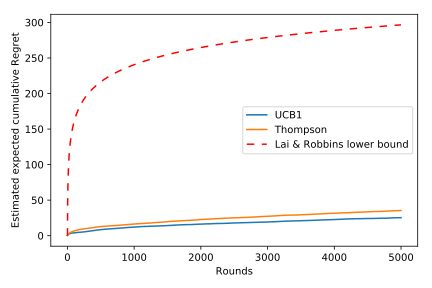
\includegraphics[width=\textwidth]{ex1_bernoulli_regret_2}
  %     \caption{Estimated expected cumulative regret for UCB1 and TS,
  %       and Lai-Robbins lower bound}\label{fig:ex1-bernoulli-arms-regret-2}
  %   \end{subfigure}
  %   \caption{Representation of the arms means and expected cumulative
  %     regret for the second chosen Bernoulli bandit}\label{fig:ex1-bernoulli-2}
  % \end{figure}
